\documentclass[12pt]{article}
\setlength\parindent{0pt}
\usepackage{fullpage}
\usepackage[margin=0.5in]{geometry}
\usepackage{amsmath}
\usepackage{graphicx}
\setlength{\parskip}{1.5em}
\def\LL{\left\langle}   % left angle bracket
\def\RR{\right\rangle}  % right angle bracket
\def\LP{\left(}         % left parenthesis
\def\RP{\right)}        % right parenthesis
\def\LB{\left\{}        % left curly bracket
\def\RB{\right\}}       % right curly bracket
\def\PAR#1#2{ {{\partial #1}\over{\partial #2}} }
\def\PARTWO#1#2{ {{\partial^2 #1}\over{\partial #2}^2} }
\def\PARTWOMIX#1#2#3{ {{\partial^2 #1}\over{\partial #2 \partial #3}} }
\newcommand{\BI}{\begin{itemize}}
\newcommand{\EI}{\end{itemize}}
\newcommand{\BE}{\begin{displaymath}}
\newcommand{\EE}{\end{displaymath}}
\newcommand{\BNE}{\begin{equation}}
\newcommand{\ENE}{\end{equation}}
\newcommand{\BEA}{\begin{eqnarray}}
\newcommand{\EEA}{\nonumber\end{eqnarray}}
\newcommand{\EL}{\nonumber\\}
\newcommand{\la}[1]{\label{#1}}
\newcommand{\ie}{{\em i.e.\ }}
\newcommand{\eg}{{\em e.\,g.\ }}
\newcommand{\cf}{cf.\ }
\newcommand{\etc}{etc.\ }
\newcommand{\Tr}{{\rm tr}}
\newcommand{\etal}{{\it et al.}}
\newcommand{\OL}[1]{\overline{#1}\ } % overline
\newcommand{\OLL}[1]{\overline{\overline{#1}}\ } % double overline
\newcommand{\OON}{\frac{1}{N}} % "one over N"
\newcommand{\OOX}[1]{\frac{1}{#1}} % "one over X"



\begin{document}
\Large
\centerline{\sc{Recitation Exercises - Rotational Kinetic Energy}}
\normalsize
\centerline{\sc{Week 12, Day 1}}

\pagenumbering{gobble}

\begin{enumerate}

\item {Formula One race cars use a ``kinetic energy recovery system'' that stores energy in rapidly spinning wheels called flywheels. When the car slows down to make a turn, the car couples the flywheel to the transmission; it begins to spin rapidly, storing some of the car's translational kinetic energy in its rotation. One type of these systems uses a flywheel of mass $m=5$ kg and radius $r=12$ cm that rotates at up to 60,000 revolutions/minute.

You can model the flywheel as a uniform cylinder ($I=\frac{1}{2}mr^2$).


a) What is its angular velocity in radians per second?

\vspace{2in}

b) How much energy does it store when rotating at full speed?

\vspace{2in}

c) Suppose the wheel is only spinning at half speed (30,000 rpm). What fraction of its maximum energy does it store? \textit{(You should be able to answer this without a calculator. If you are not sure how, ask your instructors for advice.)}

\vspace{0.5in}

d) When the car accelerates again, this system uses the rotational energy stored in the flywheel to supplement the engine power. If the system provides 100 kW of extra power, how many seconds of ``boost power'' can the system deliver before it is out of energy?

}

\newpage

\item {

As we did in class, consider rolling different objects down a slope of height $h$. In this exercise, you will determine how fast they are moving (their final speed $v$) when they reach the bottom.

First, consider a solid cylinder of mass $m$ and radius $r$. 

For each of the following, your group should guess whether it will be moving \textit{faster, slower, or the same speed} than the original cylinder when it reaches the bottom. You haven't done any calculations yet, so you may not know for sure -- that's okay! Record the result you expect and a brief reason why.

\begin{itemize}
\item A more massive solid cylinder of mass $2m$ with the same radius $r$
\item A larger solid cylinder with the same mass $m$, but with radius $2r$
\item A hollow cylinder, also of mass $m$ and radius $r$
\item A solid sphere, also of mass $m$ and radius $r$
\end{itemize}

\vspace{0.4in}

Now, we'll calculate how fast each of them go down the slope. First, consider a hollow cylinder rolling down the slope. As it rolls, its potential energy at the top is converted into kinetic energy. You may write things in terms of $g$, $m$, $r$, $h$, etc. here; we don't have any numbers.

\begin{enumerate}
	\item What is its total energy at the top of the slope?
\vspace{0.7in}

    \item What is its total energy at the bottom of the slope? (Hint: What kinds of energy does it have there?)
    
    \vspace{1in}
    
    \item If you set these two expressions for the total energy equal (since no other force does work here, and since energy is conserved), you will arrive at an equation that you could solve for $v$, the speed that the ball is moving at the bottom. However, it has another unknown in it: $\omega$, the rate at which it is rotating.
    
    However, the ball is rolling without slipping. What condition relates $v$ to $\omega$ if the ball rolls without slipping?
    
    \vspace{1in}
    \newpage
    
    \item Make this substitution, and arrive at an expression for $v$. What does it depend on? What does it not depend on?
    
    \vspace{2.5in}
    
    Now, we'll consider objects other than a hollow cylinder: a solid ball, a solid cylinder, and a hollow ball. These will have different forms for the moment of inertia: instead of $I=mr^2$, their moments of inertia have the form $I=\lambda mr^2$, where $\lambda$ is a fraction. 
    
    We could do these calculations one at a time, but it is much faster to do the calculation leaving $\lambda$ in the expression for $I$; then you can substitute in at the end.
    
    Repeat the above calculation for all of these other shapes. You'll arrive at a general formula for the speed of an object (whatever its shape) of mass $m$ and radius $r$ after rolling down a hill of height $h$.
    
    \vspace{3in}
    
    \vfill Check your result with your TA once you have it.
    
    \newpage
    
    \item Here's our list of objects again.
    
\begin{itemize}
	\item A solid cylinder of mass $m$ and radius $r$
	\item A more massive solid cylinder of mass $2m$ with the same radius $r$
	\item A larger solid cylinder with the same mass $m$, but with radius $2r$
	\item A hollow cylinder, also of mass $m$ and radius $r$
	\item A solid sphere, also of mass $m$ and radius $r$
\end{itemize}
    
    Rank them in order of how quickly they'll be moving when they reach the bottom of the ramp. Think about which quantities ($m$, $r$, and the shape) appear in your formula and which don't.
    
\end{enumerate}
}

\vspace{3in}

\item In the previous exercise, you arrived at a formula for $v_f$ in terms of $g$, $h$, and $\lambda$.

\bigskip\bigskip

Suppose that you have some other ramp. You observe that when you roll a hollow sphere down it, it's traveling at 1 m/s. How fast would a solid sphere be traveling? \textit{(You do have enough information to provide a number here, even though you don't know $m$, $g$, $h$, or $r$.)}


\end{enumerate}

\newpage


\begin{center}
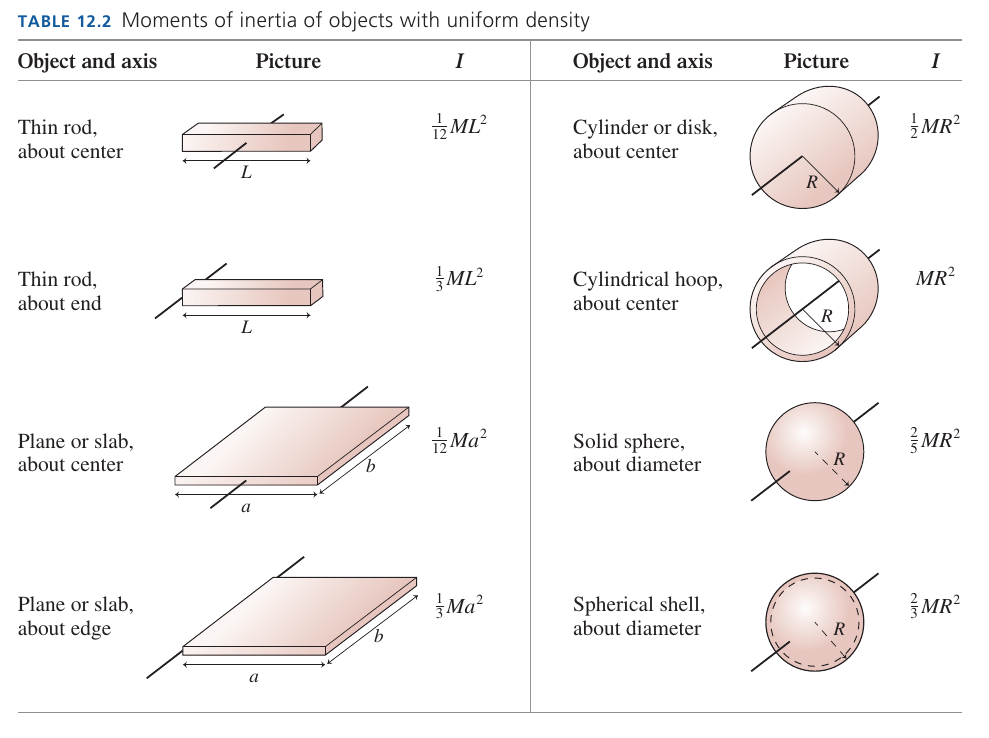
\includegraphics[width=7in]{moment-table.png}
\end{center}

\end{document}
